\chapter{State of the art}
\label{chap:sota}
The technique of
mixing real world elements with virtual elements displayed on the screen of a
device is what we call augmented reality. In the field of augmented reality, a
lot of things have happened during the last years. The progress in the fields
of computer vision and image processing have led to several new techniques of
detection and tracking. This, combined with the increasing availability of
powerful mobile devices, has enabled developers to build a plethora of high
quality AR-based applications. Nowadays, modern mobile devices use integrated
cameras, motion sensors and proximity sensors to make these AR-based experiences. 

Augmented reality in mobile devices is slightly different from what can be seen in
desktop environments. Although every year we have more powerful mobile
smart-phones, processing and drawing into the device's screen is still an 
expensive operation in terms of computational cost. This is one of the reasons why
cost-efficient computer vision algorithms and techniques have emerged in the recent
years. 

Most of the augmented reality apps follow this behavior:
\begin{itemize}
\item Get the input from the camera or a video.
\item Search for an object of interest.
\item Introduce our object into the scene, considering the camera or the input position.
\end{itemize}

In this chapter we are going to describe which are the different techniques
that enables us to do this kind of processing, but before that we need to
explain some key concepts. 

We call \emph{source image} or \emph{source object} to the image used as the pattern
that the algorithm is searching for in the scene. Depending on the source image, the
algorithms tested will perform better or worst. We define \emph{robustness} as the
quality of a tracking 
algorithm when the scene changes and the object to track is not equal as the
source image. This difference between the image to track and the image
presented in the camera can be due to \emph{rotation}, \emph{scale} or
\emph{perspective transformation}. Some algorithms described below are
unaffected to some of this changes. For instance, being \emph{rotation
  invariant} means that the algorithm is \emph{robust} enough to still
recognize the object in the scene despite of its rotation difference between
the original object.

Before starting to
introduce this technologies, it is interesting to explain the frame rate
reference of 60 FPS and why is the main goal of many graphics visual
applications.
Douglas Trumbull introduced the 60 frames per second rate as the most
convenient for human eye while developing Showscan, his cinematic process. The
main reason for achieving this performance is that it enables a better
emotional connection with the viewer because the frame rate is higher than the
regular 24 FPS used in 35mm film. Trumbull ran laboratory tests with
electroencephalograms and electrocardiograms when projecting 24, 36, 48, 60, 66, and
72 FPS films to viewers~\cite{trumbull}. The result was that the stimulus when 
viewing 60 frames per second films was higher than others.
Although the goal is to achieve 60 frames per
second, the human eye perceives sloppiness at frame rates lower than 20 FPS, so
getting a higher value than that is considered enough for most applications.

The goal of this work is to find a combination of techniques that enable us to
develop an application with object tracking invariant to rotation, scale and
perspective warp. The different algorithms tested were selected with this target
in mind. 

\section{Object recognition}
In order to provide an augmented reality experience, we have to know first
which is the real world element that we are going to use as a reference to mix
the real world input with our virtual elements. This reference can be from an
image from the smart-phone camera to the user location. Our application searches a
particular image inside the camera input in order to draw the poster image
above. Many other augmented reality mobile apps do not necessarily use image
processing techniques to mix real world elements with virtual ones. For
instance, there are applications that helps the user to identify constellations
with the mobile phone. These applications only use GPS location and digital
compass orientation to enable the user to see which constellations are they
pointing their device to.

The technique of searching an image and follow it along it's 
movement is usually referred as object tracking. 
In computer vision there are a lot of object recognition techniques. In the
development of Ponster, two of these techniques have been tested: template
matching and feature-based detection. Detecting the image in a continuous input from
the smart-phone camera, taking account of scale, rotation and perspective
differences, becomes an object tracking technique. 

\section{Template matching}
Template matching\cite{ocv01} consists of finding areas of an image that are similar to a
provided template image. We have to set as the input of the algorithm a template
image ---the image that we want to look for--- and compare it with the source image
---the image in which we want to search\cite{tmatch01}---. Template matching is also
called area-based approach. 

OpenCV provides a way to perform template matching with several methods, such as
square difference matching\footnote{\texttt{SQDIFF}.} or correlation-matching
methods\footnote{\texttt{CCORR}.}. With the latest, \texttt{CCORR}, we use a 
correlation formula to check if the template is inside the image. Instead of
applying a yes/no approximation, we can bring a positive match with a certain
threshold. 

\begin{figure}
\centering
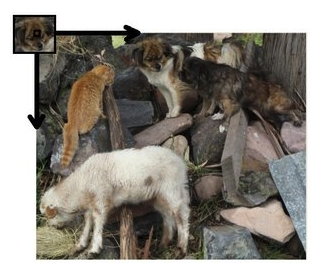
\includegraphics[scale=0.75]{img/templatematch.png}
\caption{\label{fig:templatematch}How the template matching algorithm works in
  OpenCV. Taken from
  \url{http://docs.opencv.org/doc/tutorials/imgproc/histograms/template_matching/template_matching.html}} 
\end{figure} 

% citar el ppt aquel
Performing a template matching operation using OpenCV on mobile devices is fast
enough to deliver a smooth 25/30 FPS\footnote{Frames per second.}-like
detection. However, match template does not 
take account of scale, rotation and perspective invariance by itself. There are
several approaches to bring invariance to match template. For instance, image
pyramids are used to make match template scale and rotation
invariant\cite{4368176}, but it is not part of the OpenCV match template function, although it
provides some methods to implement image pyramids\cite{ocv02}. A visual
representation of an image pyramid can be seen in figure~\ref{fig:pyramid}. 

\begin{figure}
\centering
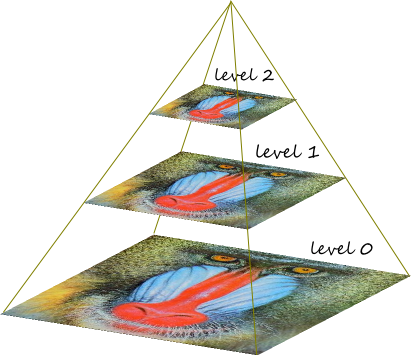
\includegraphics[scale=0.65]{img/pyramid.png}
\caption{\label{fig:pyramid}An example of image pyramid technique. Taken
  from~\cite{imgpyramid}.} 
\end{figure} 

In the testing of template matching in Ponster, a basic image pyramid algorithm
has been developed. Our simple image pyramid algorithm consists of building
several sizes of the pattern image provided to the app. We generate four
smaller versions of the image and then we try to match them in each frame of
the camera loop. If any of the images is detected, we take account of the
image scale to draw the poster above the detected pattern. In our tests this
worked really well, but more scale images were needed to bring a better scale
invariance template matching algorithm.

Match template has been tested during the development of Ponster. Also, a basic
image pyramid system has been developed for scale-invariance, but match template has
been discarded in favor of feature detection algorithms because they bring rotation
 invariance and perspective warp, and this are required features to deliver a
 good augmented reality experience.

\section{Feature detection}
A feature-based approach can be presented as a three step method. First of all, we
have to detect keypoints\cite{feature} ---also called interest points--- in the
image. Usually, 
interest points are corners, blobs\footnote{Regions and points that have
  different brightness, color or contrast compared with their neighbor
  region.} or junctions ---see figure~\ref{fig:junctions}---. A good keypoint is a 
\emph{repeatable} keypoint; if we can find the same keypoint under different
conditions such as light difference or rotation, it's considered as a quality
keypoint. The second step is to compute \emph{descriptors} or feature
vectors. These descriptors are represented as neighborhoods of interest
points. Assuming that feature
detection makes sense when we have two images to compare, these two steps have to be
performed on both images. Once we've done that, we have a group of descriptors for
each image, and we have to compare them in order to \emph{match} features. If the
features of the source image are present in the input image, we can assume that the
object has been detected. The matching is based on the distance between the feature
vectors. 

\begin{figure}
\centering
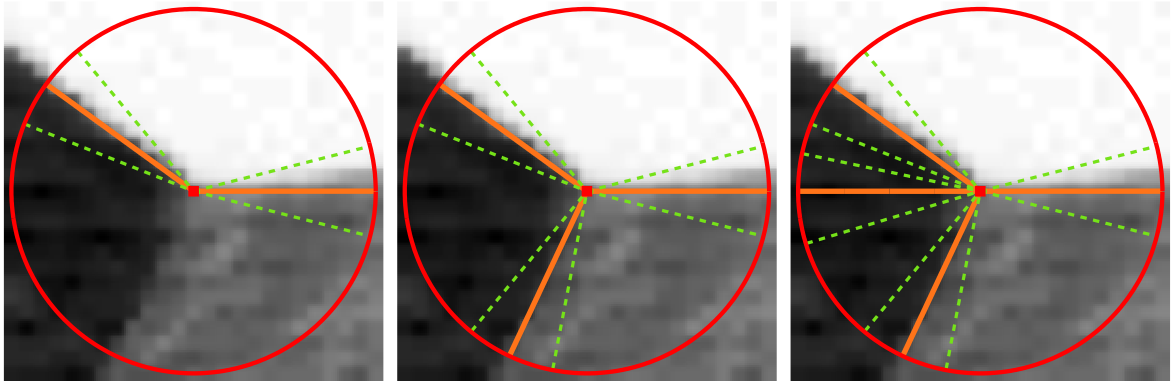
\includegraphics[scale=0.25]{img/junction.png}
\caption{\label{fig:junctions}Different types of junctions, taken
  from~\cite{junction}.} 
\end{figure} 

Usually, source images with enough keypoints are easier to detect than more
uniform images. This is why it's better to select a good source image with many
features and good contrast. 
As we've said before, in order to deliver a good augmented reality experience,
we need to make our detection algorithm scale, rotation and perspective
invariant. Feature detection techniques can be scaled invariant by extracting
features that are invariant to scale, such as feature vectors computed from
interest point neighborhoods. For rotation invariance, algorithms can
estimate the orientation of the keypoint. % and for perspective 

%TODO introduce following chapters
There are plenty of feature-detection based algorithms, many of them based on
Scale-Invariant Feature Transform, or SIFT. Cost efficiency is one of the most
important features of these algorithms, as every new technique introduced tries to
maintain robustness while reducing computation time. Robustness it's also very
important, but less robust algorithms are also been developed in favor of more
efficient techniques. One good example is FAST\cite{6126544} keypoint detector, which is
not rotation invariant but it's faster to compute.

Next, we are going to describe the feature-detection algorithms tested during the
development of Ponster: SURF, FREAK and ORB.

\subsection{Speeded-Up Robust Features - SURF}
Speeded-Up Robust Features ---also know as SURF--- is a group of detector and descriptor
introduced by Herbert Bay et al. SURF is faster and more robust than other
alternatives like SIFT\cite{Bay:2008:SRF:1370312.1370556}. Its descriptors are
rotation and scale invariant. Perspective transformations are also considered, but
in lower order.  

The keypoint detection in SURF uses a Hessian-matrix approximation. This use of
integral images reduces computational cost in comparison with another interest point
detection techniques such as Harris corner detection. Scale invariance is achieved
by calculating integral image pyramids, but instead of reducing the image size,
integral images allow SURF to upscale and build the pyramids more efficiently. 

The SURF descriptor calculation is slightly based on SIFT. SURF descriptor describes
the distribution of the intensity content within the interest point neighborhood,
which is similar to the gradient information used by SIFT. It is done in two steps,
fixing a reproducible orientation based on information from a circular region around
the keypoint, and then building a square region aligned to the calculated
orientation. Once we have the descriptors, the last step is to perform the
matching. Descriptors are compared only if they have the same type of contrast,
allowing to perform a faster matching. In Ponster, two different matching algorithms
have been tested, Brute-force Matcher and FLANN-based matching.

SURF is as robust as other alternatives such as SIFT, but it's faster to compute due
to the use of integral images. It is rotational and scale-invariant, which is better
than the template matching technique described before, but it's performance running
on the device (iPhone 5, iOS 7.1.2 and iOS 8) is not good enough to deliver a decent user
experience, taking between 0.7 and 1 second to compute each image, as can be
seen in the performance tests in section~\ref{sec:arperf}. Also, SURF is a
patented algorithm and it's not allowed its use in commercial applications. 

\subsection{Fast Retina Keypoint - FREAK}
FREAK stands for Fast Retina Keypoint\cite{Ortiz:2012:FFR:2354409.2354903}. As we
have stated before, the trend is to make descriptors faster to compute while
remaining robust and scale, rotation invariant. FREAK uses a keypoint descriptor
designed like the human retina with this goal in mind.

Fast Retina Keypoint proposes to use a retinal sampling grid that takes account of
the higher density points near the center of the sample points. This is exactly how
the human retina works, and the FREAK sampling pattern imitates this natural
behavior~\ref{fig:freak}. With FREAK, every keypoint gets this retina sampling
pattern to compute its descriptors. Then, the algorithm compares pairs of image
intensities obtained by this pattern.

\begin{figure}
\centering
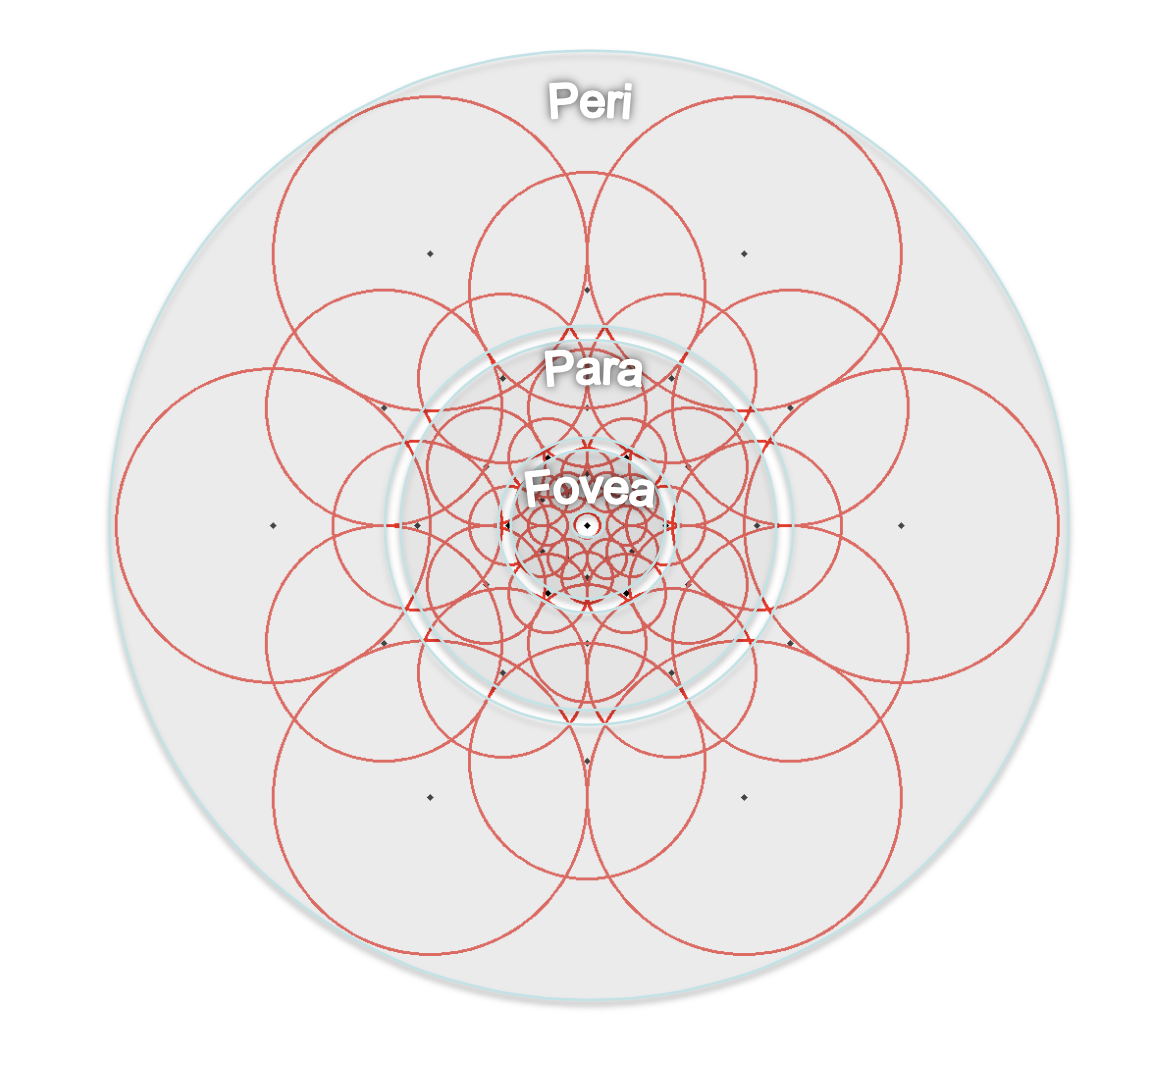
\includegraphics[scale=0.55]{img/freak.png}
\caption{\label{fig:freak}FREAK sampling pattern with it's equivalent in the human
  retina.} 
\end{figure} 

One of the main reasons of choosing FREAK to test as a descriptor combined with
SURF is that it has more robustness in term of rotation and scale
invariance than the SURF descriptor extractor. The
comparison of SURF with different descriptor 
extractor\cite{rotationscaleinv} shown in the figures~\ref{fig:surfrotation}
and~\ref{fig:surfscale}
shows that the robustness of the detection in both parameters is increased when
using FREAK. 

\begin{figure}
\centering
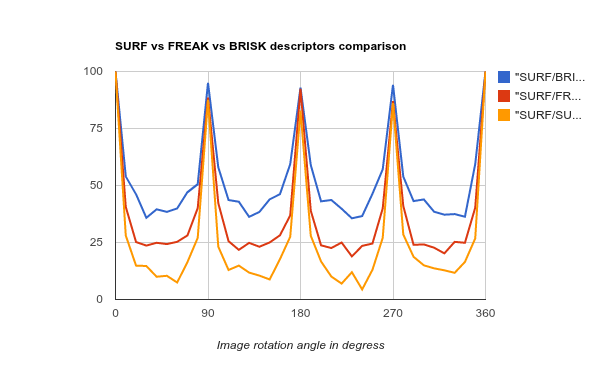
\includegraphics[scale=0.75]{img/rotation.png}
\caption{\label{fig:surfrotation} Rotation invariance comparison between different descriptor
  extractors combined with SURF. Source~\cite{rotationscaleinv}.}
\end{figure} 

\begin{figure}
\centering
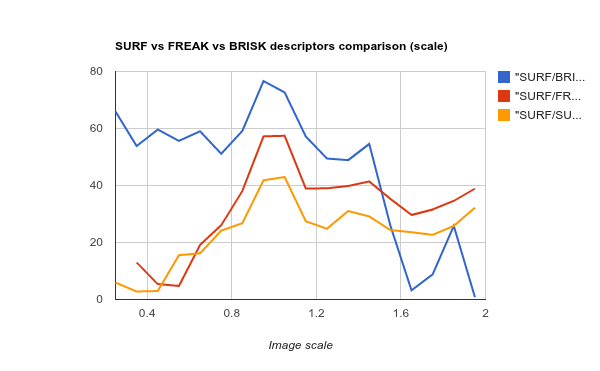
\includegraphics[scale=0.75]{img/scale.png}
\caption{\label{fig:surfscale}Scale invariance comparison between different descriptor
  extractors combined with SURF. Source~\cite{rotationscaleinv}.}
\end{figure} 

In the section~\ref{sec:arperf} we present a comparison between the three
approaches chosen for the object detection. We can clearly see that using FREAK
as the descriptor extractor can boost the performance compared with SURF
descriptors, but it also delivers less matches.

\subsection{Features from Accelerated Segment Test - FAST}
FAST is a keypoint detector based on corner detection. It was introduced by
Edward Rosten and Tom Drummond\cite{Rosten:2006:MLH:2094437.2094478} and its
primary purpose was to bring a real 
time interest point detector. FAST considers a circle of sixteen pixels around
each corner candidate, and detects a candidate as a corner if there are $n$
contiguous pixels in that circle with brighter intensity than the candidate
pixel. % introduce Figure 1 of paper [3]

This technique is faster than others for corner detection, but FAST is not
scale and rotation invariant. Also, it does not perform very well under high
noise images. Many other techniques uses FAST as a starting point of a
detector, bringing scale and rotation invariance and a corresponding
extractor. One example of this is ORB, tested in the development of Ponster.

\subsection{Oriented FAST and Rotated BRIEF - ORB}
% paper: ORB: an efficient alternative to SIFT or SURF
As we have said before, real time performance has been a very popular topic in
object detection during the last years. The main characteristic of ORB is to
perform as good as SIFT in terms of robustness, but doing it twice as fast. ORB
uses a variant of FAST as the interest point detector, and BRIEF as the
descriptor extractor.  

FAST does not have rotation invariance. This is why ORB uses oFAST (FAST
keypoint orientation), which is a variant of FAST that computes orientation by
intensity centroid. This technique assumes that a corner's intensity is offset
from its center, and this vector may be used to impute an
orientation\cite{6126544}. To bring scale invariance, ORB employs a scale pyramid of
the image and computes FAST on each level of the pyramid.

ORB also uses a variant of BRIEF called rBRIEF, or Rotation-aware BRIEF. The
BRIEF descriptor, unlike SURF, is a binary descriptor. rBRIEF is based on
steered BRIEF, which uses the keypoint orientation; in addition to steered
BRIEF, a learning method for choosing good binary features is applied,
resulting into rBRIEF.

In Ponster, ORB has been tested with better results than the other previous
techniques, but again with poor performance in the device\footnote{We can
  consider poor performance a FPS under 20.}. Only a 15 FPS
processing has been achieved, with slightly the same detection quality as
SURF, as it can bee seen in the chapter~\ref{sec:arperf}. It is interesting to
note that, although each of the algorithms tested 
are scale invariant, they tend to lose the tracked image when the scale of the object
represented in the camera feed is 50\% smaller than the original. This is also
happening with SURF-SURF and SURF-FREAK combinations~\ref{fig:surfscale}.

\section{Matching}
Once we have calculated the interest points and computed the descriptors in the
two images that we want to compare, we have to perform a match between this two
sources. Depending on the descriptor extraction method, one or another matcher
must be used. ORB uses binary descriptors, but SURF does not, so the matching
is performed in a different way.

We will discuss two of this methods, both used in the development of Ponster,
Brute-force matcher and Fast Library for Approximate Nearest Neighbors. 

\subsection{Brute-Force Matcher}
%features.ppt hay una buena imagen
% mirar Fast Matching of Binary Features
Brute-Force Matcher, as it's name states, will compare each of the descriptors
found in the images, thus performing a linear search. Although it may seem that
this approach is not very efficient, BF-matcher performs really well on binary
descriptors like ORB. 

The comparison is done by a distance function. There are many functions in
BF-matcher:
\begin{itemize}
\item \texttt{NORM\_L1} better with SURF/SIFT.
\item \texttt{NORM\_L2} better with SURF/SIFT.
\item \texttt{NORM\_HAMMING} better with ORB.
\item \texttt{NORM\_HAMMING2} better with ORB.
\end{itemize}
Hamming distance can be computed with bit manipulation operations, which are
very quick. In Ponster, Hamming distance has been tested for ORB and L2
normalization with SURF. 

\subsection{Fast Library for Approximate Nearest Neighbors - FLANN}
Instead of performing a linear search for matching descriptors, we can use a
nearest neighbor matching technique. The nearest neighbor search tries to
find, given a set of points $P$ in a vector space $X$, all the points that are 
close to a given point $q$. FLANN\cite{muja:fast}
is a library that enables us to perform this
kind of searches with several algorithms. Two have been tested in Ponster,
randomized KD-tree search for SURF and Locality-Sensitive Hashing for ORB.

\subsubsection{Randomized KD-tree}
Basic KD-tree search performs well for small datasets, but quickly degrades
its performance when the dimensionality increases. In order
to reduce the computational cost of KD-tree searches with large datasets, several
KD-tree algorithm variants have been introduced, such as approximate nearest
neighbor. 

This algorithm creates multiple randomized KD-trees, built by choosing the
split dimension randomly from the first $5$ dimensions on which data has the
greatest variance. Then, a priority queue is created while searching all the
trees, so the search can be ordered by increasing distance to each bin
boundary. 

Using this approximation techniques can boost performance by reducing the
precision of the matching, although the loss is usually small enough to maintain
a $95\%$ precision. 

\subsubsection{Locality-Sensitive Hashing}
Locality-Sensitive Hashing is a matching algorithm to solve the nearest
neighbor search in high datasets. LSH is used with binary descriptors like the
ones computed with ORB. The main idea of LSH is to hash the points with
functions that ensure that close points will be more likely to key collision,
thus allowing to get the nearest neighbors of each point querying the other
points in it's bucket\cite{Andoni:2008:NHA:1327452.1327494}.

The LSH parameters defines the hash functions \emph{amplification}. This means that
the hash functions must be \emph{amplified} enough to ensure hash collision;
otherwise, the algorithm would be useless. The effect of this parameters and a more
in-depth explanation of LSH can be found in
this~\cite{Andoni:2008:NHA:1327452.1327494} paper. 

\section{Natural feature tracking}
\label{sec:naturalfeature}
Although the technologies explained in previous sections are robust and reliable,
and have been successfully tested, they have not been used in the last version of
Ponster due to it's poor performance on mobile devices. Another technique has been proven
to be successful to deliver both high performance in mobile devices and robust
object tracking.

Natural feature tracking consists of computing the motion of a feature in the
scene\cite{neumann}. We call nature feature to any point or
region candidate to be detected and selected as a reference. Usually this
follows the next steps: 
\begin{itemize}
\item Natural feature detection and selection.
\item Motion estimation based on detected features.
\item Evaluation feedback for stabilized detection and tracking.
\end{itemize}
The feature detection consists in selecting points and regions in the image
with specific characteristics that are easy and robust to track. The motion
estimation can be executed by several ways. For example, in Neumann's
paper~\cite{neumann}, optical  
flux is presented to estimate the camera movement. In our mobile environment,
we can also use the built-in gyroscope of the iPhone 5. The evaluation feedback provides a way to reject
detected features that do not specifically match with the plane that should be
representing, thus allowing the algorithm to avoid false positives and do not
corrupt the tracking output.

The technology used in Ponster to perform the augmented reality is called
Vuforia and uses Natural feature tracking to track the object in the scene. In
the section~\ref{sec:vuforia} we describe how Vuforia works, although it is a
propietary solution and thus we cannot have detailed information about how
internally does the tracking. 
